\documentclass{article}
\usepackage{alltt}
\usepackage{casl}
\usepackage{xspace}
\usepackage{color}

\input{xy}
\xyoption{v2}

\newcommand{\QUERY}[1]%{}
{\marginpar{\raggedright\hspace{0pt}\small #1\\~}}

\newcommand{\eat}[1]{}

\newenvironment{EXAMPLE}[1][]   {\par#1\begin{EXAMPLEFORMAT}\begin{ITEMS}}
                                {\end{ITEMS}\end{EXAMPLEFORMAT}\par}
\newcommand{\IEXT}[1]           {\\#1\I}
\newcommand{\IEND}              {\I\END}
\newenvironment{EXAMPLEFORMAT}  {}{}

%% Added by MB to have some extra vertical space after the ``main'' examples
%% following the points (and some others in the text): 
\newenvironment{BIGEXAMPLE}   {\begin{EXAMPLE}} {\end{EXAMPLE}\medskip}
\newenvironment{DETAILS}[1][]   {#1\begin{DETAILSFORMAT}}{\end{DETAILSFORMAT}}
\newenvironment{DETAILSFORMAT}  {}{}
\newenvironment{META}[1][]      {#1\begin{METAFORMAT}}{\end{METAFORMAT}}
\newenvironment{METAFORMAT}     {\medskip\vrule\hspace{1ex}\vrule\hspace{1ex}%
                                 \begin{minipage}{0.9\textwidth}\it}
                                {\end{minipage}\par\medskip}

\newcommand{\SLIDESMALL}        {}
\newcommand{\SLIDESONLY}[1]     {}


%%%%%%%%%%%%%%%%%%%%%%%%%%%%%%%%%%%%%%%%%%%%%%%%%%%%%%%%%%%%%%%%%%%%%%
% SIMULATING SMALL-CAPS FOR BOLD, EMPH

\newcommand{\normalTEXTSC}[2]{{#1\scriptsize#2}}
%% NOT \newcommand{\normalTEXTSC}[2]{{\normalsize#1\scriptsize#2}}
\newcommand{\largeTEXTSC} [2]{{\large     #1\small     #2}}
\newcommand{\LargeTEXTSC} [2]{{\Large     #1\normalsize#2}}
\newcommand{\LARGETEXTSC} [2]{{\LARGE     #1\large     #2}}
\newcommand{\hugeTEXTSC}  [2]{{\huge      #1\Large     #2}}
\newcommand{\HugeTEXTSC}  [2]{{\Huge      #1\LARGE     #2}}


%\newcommand     {\CASL}{\normalTEXTSC{C}{ASL}\xspace}
\newcommand{\largeCASL} {\largeTEXTSC{C}{ASL}\xspace}
\newcommand{\LargeCASL} {\LargeTEXTSC{C}{ASL}\xspace}
\newcommand{\LARGECASL} {\LARGETEXTSC{C}{ASL}\xspace}
\newcommand {\hugeCASL}  {\hugeTEXTSC{C}{ASL}\xspace}
\newcommand {\HugeCASL}  {\HugeTEXTSC{C}{ASL}\xspace}

%\newcommand     {\CoFI}{CoFI\xspace}

\newcommand     {\MAYA}{\normalTEXTSC{M}{AYA}\xspace}
\newcommand{\largeMAYA} {\largeTEXTSC{M}{AYA}\xspace}

\newcommand     {\Hets}{\normalTEXTSC{H}{ETS}\xspace}
\newcommand{\largeHets} {\largeTEXTSC{H}{ETS}\xspace}
\newcommand{\LARGEHets} {\LARGETEXTSC{H}{ETS}\xspace}

\newcommand     {\Cats}{\normalTEXTSC{C}{ATS}\xspace}
\newcommand{\largeCats} {\largeTEXTSC{C}{ATS}\xspace}

\newcommand     {\ELAN}{\normalTEXTSC{E}{LAN}\xspace}
\newcommand{\largeELAN} {\largeTEXTSC{E}{LAN}\xspace}

\newcommand     {\HOL}{\normalTEXTSC{H}{OL}\xspace}
\newcommand{\largeHOL} {\largeTEXTSC{H}{OL}\xspace}

\newcommand     {\Isabelle}{\normalTEXTSC{I}{SABELLE}\xspace}
\newcommand{\largeIsabelle} {\largeTEXTSC{I}{SABELLE}\xspace}

\newcommand     {\Horn}{\normalTEXTSC{H}{ORN}}

%%%%% Klaus macros
\newcommand{\CASLDL}{\textmd{\textsc{Casl-DL}}\xspace}
\newcommand{\Dolce}{\textmd{\textsc{Dolce}}\xspace}
\newcommand{\SHOIN}{$\mathcal{SHOIN}$(\textbf{D})\xspace}
%%%%% end of Klaus macros

%% Use \ELAN-\CASL, \HOL-\CASL, \Isabelle/\HOL

\newcommand{\LCF}{LCF\xspace}

\newcommand{\ASF}{ASF\xspace}
%%\newcommand     {\ASF}{\normalTEXTSC{A}{SF}\xspace}
%%\newcommand{\largeASF} {\largeTEXTSC{A}{SF}\xspace}

\newcommand{\SDF}{SDF\xspace}
%%\newcommand     {\SDF}{\normalTEXTSC{S}{DF}\xspace}
%%\newcommand{\largeSDF} {\largeTEXTSC{S}{DF}\xspace}

\newcommand     {\ASFSDF}{\normalTEXTSC{A}{SF}+\normalTEXTSC{S}{DF}\xspace}
\newcommand{\largeASFSDF} {\largeTEXTSC{A}{SF}+\largeTEXTSC{S}{DF}\xspace}

\newcommand     {\HasCASL}{\normalTEXTSC{H}{AS}\normalTEXTSC{C}{ASL}\xspace}
\newcommand{\largeHasCASL} {\largeTEXTSC{H}{AS}\largeTEXTSC{C}{ASL}\xspace}

%% Do NOT use \ASF+\SDF (it gives a superfluous space in the middle)

\newcommand{\CCC}{CCC\xspace}

\newcommand{\CoCASL}{\normalTEXTSC{C}{O}\normalTEXTSC{C}{ASL}\xspace}
\newcommand{\CspCASL}{\normalTEXTSC{C}{SP}-\normalTEXTSC{C}{ASL}\xspace}
\newcommand{\Csp}{\normalTEXTSC{C}{SP}\xspace}
\newcommand{\CcsCASL}{CCS-\normalTEXTSC{C}{ASL}\xspace}
\newcommand{\CASLLtl}{\normalTEXTSC{C}{ASL}-\normalTEXTSC{L}{TL}\xspace}
\newcommand{\CASLChart}{\normalTEXTSC{C}{ASL}-\normalTEXTSC{C}{HART}\xspace}
\newcommand{\SBCASL}{\normalTEXTSC{S}{B}-\normalTEXTSC{C}{ASL}\xspace}
\newcommand{\HetCASL}{\normalTEXTSC{H}{ET}\normalTEXTSC{C}{ASL}\xspace}
\newcommand{\ModalCASL}{\normalTEXTSC{M}{odal}\normalTEXTSC{C}{ASL}\xspace}


\begin{document}

\title{{\bf \protect{\LARGEHets} User Guide}\\ 
-- Version 0.44 --}
\author{Till Mossakowski\\[1em]
Department of Computer Science\\ and Bremen
Institute for Safe Systems,\\ University of Bremen, Germany.\\[1em]
Comments to: hets@tzi.de
}

\maketitle

\section{Introduction}


The Heterogeneous Tool Set (\protect\Hets) is the main analysis tool
for the specification language heterogeneous \CASL. Heterogeneous
\CASL (\HetCASL) combines the specification language \CASL with \CASL extensions
and sublanguages, as well as completely different logics and even
programming languages such as Haskell. \HetCASL
extends the structuring mechanisms of \CASL:
\emph{Basic specifications} are
unstructured specifications or modules written in a specific logic.
The graph of currently supported logics is shown in Fig.~\ref{fig:LogicGraph},
and the degree of support by \Hets in Fig.~\ref{fig:Languages}.

With \emph{heterogeneous structured specifications}, it is possible to
combine and rename specifications, hide parts thereof, and also
translate them to other logics. \emph{Architectural specifications}
prescribe the structure of implementations.  \emph{Specification
  libraries} are collections of named structured and architectural
specifications. 

\Hets consists of logic-specific tools for the parsing and static
analysis of the different involved logics, as well as a
logic-independent parsing and static analysis tool for structured and
architectural specifications and libraries. The latter of course needs
to call the logic-specific tools whenever a basic specification is
encountered.

\section{Logics supported by \Hets}

\begin{figure}
  \begin{center}
    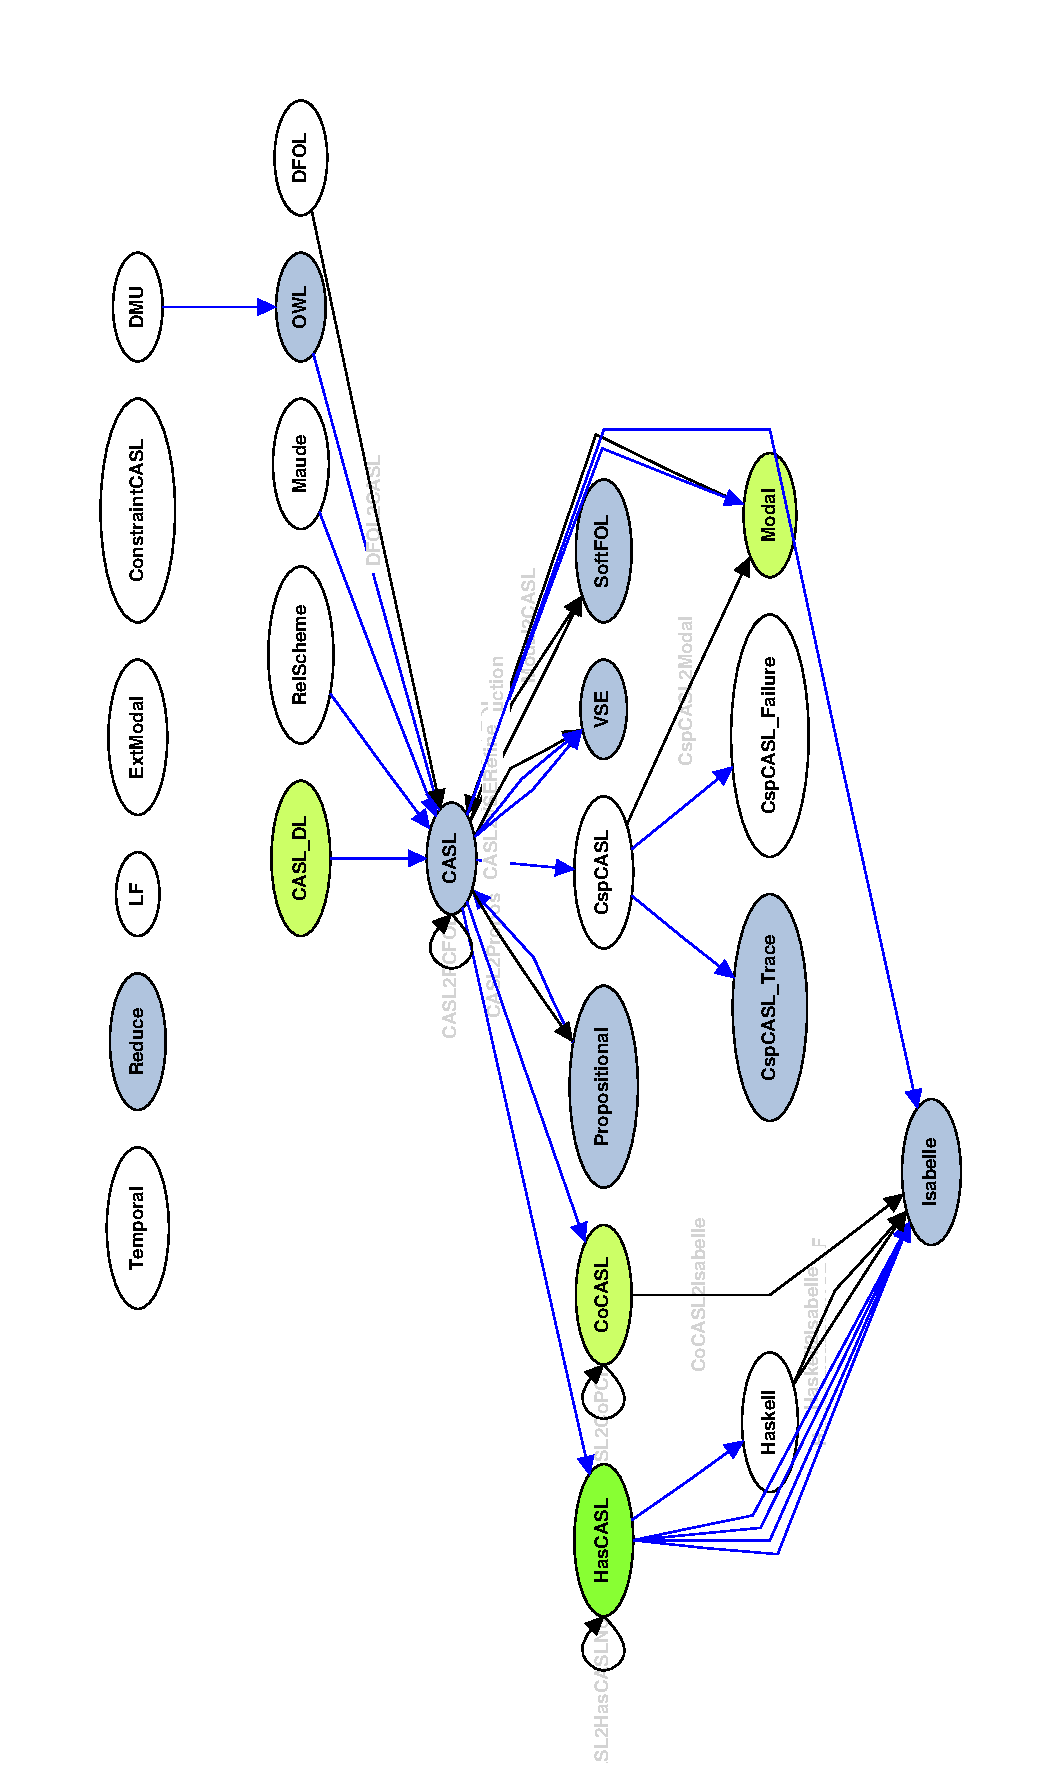
\includegraphics[scale=0.4]{LogicGraph}
  \end{center}
\caption{Graph of logics currently supported by \Hets. The more an 
ellipse is filled, the more stable is the implementation of the logic.}
\label{fig:LogicGraph}
\end{figure}


\begin{figure}
\begin{center}
\begin{tabular}{|l|c|c|c|}\hline
Language & Parser & Static Analysis & Prover \\\hline
\CASL & x & x & - \\\hline
\CoCASL & x & x & - \\\hline
\ModalCASL & x & x & - \\\hline
\HasCASL & x & (x) & - \\\hline
Haskell & x & x & -\\\hline
\CspCASL & (x) & - & - \\\hline
%Structured specifications & x & x & (x) \\\hline
%Architectural specifications & x & x & -\\\hline
\CASLDL & x & - & - \\\hline
OWL DL basic & x & (x) & - \\\hline
OWL DL structure & x & (x) & - \\\hline
SPASS & - & - & x \\\hline
Isabelle & - & - & x \\\hline
\end{tabular}
\end{center}
\caption{Current degree of \Hets support for the different languages.\label{fig:Languages}}
\end{figure}

\begin{description}
  
\item[CASL] extends many sorted first-order logic with partial
  functions and subsorting.  It also provides induction sentences,
  expressing the (free) generation of datatypes.
%It is mainly designed and used for the
%specification of requirements for software systems. But it is also
%used for the specification of \Dolce (Descriptive Ontology for
%Linguistic and Cognitive Engineering), an Upper Ontology for knowledge
%representation. \cite{Gangemi:2002:SOD} Further it is now used to
%specify calculi for time and space. 
For more details on \CASL see \cite{CASL-RM,CASL-UM}.
%
We have implemented the \CASL logic in such a way that much of the
implementation can be re-used for \CASL extensions as well; this
is achieved via ``holes'' (realized via polymorphic variables) in the
types for signatures, morphisms, abstract syntax etc.  This eases
integration of \CASL extensions and keeps the effort of integrating
\CASL extensions quite moderate.

\item[CoCASL] \cite{MossakowskiEA04} is a coalgebraic extension of \CASL,
suited for the specification of process types and reactive system.
The central proof method is coinduction.

\item[ModalCASL] is an extension of \CASL with multi-modalities and
term modalities. It allows the specification of modal systems with 
Kripke's possible worlds semantics. It is also possible to express
certain forms of dynamic logic. 

\item[HasCASL] is a higher order extension of \CASL allowing
  polymorphic datatypes and functions. It is closely related to the
  programming language Haskell and allows program constructs being
  embedded in the specification. 
  An overview of \HasCASL is given in \cite{Schroeder:2002:HIS};
the language is summarized in \cite{HasCASL/Summary}.
The latter document is also available on the CD-ROM 
in \texttt{Tools/Hets/doc}.

\item[Haskell] is a modern, pure and strongly typed functional
  programming language. It simultaneously is the implementation
  language of \Hets, such that in the future, \Hets might be applied
  to itself.
The definitive reference for Haskell is \cite{PeytonJones03},
see also \url{www.haskell.org}. 
  
\item[CspCASL] \cite{Roggenbach:2003:C-CN} is a combination of \CASL
  with the process algebra CSP.

\item[OWL DL] is the Web Ontology Language (OWL) recommended by the
  World Wide Web Consortium (W3C, \texttt{http://www.w3c.org}). It is
  used for knowledge representation and the Semantic Web
  \cite{berners:2001:SWeb}. 
Hets calls an external OWL DL parser
  written in JAVA to obtain the abstract syntax for an OWL file and its
  imports. The JAVA parser is also doing a first analysis classifying
  the OWL ontology into the sublanguages OWL Full, OWL DL and OWL
  Lite. 
 Hets only supports the last two, more restricted variants. 
The
  structuring of the OWL imports is displayed as Development Graph.

\item[CASL-DL] is an extension of a restriction of \CASL, realizing
a strongly typed variant of OWL DL in \CASL syntax.
It extends
  \CASL with cardinality restrictions for the description of sorts and
  unary predicates. The restrictions are based on the equivalence
  between \CASLDL, OWL~DL and \SHOIN. Compared to \CASL only unary
  and binary predicates, predefined datatypes and concepts (subsorts
  of the topsort Thing) are allowed. It is used to bring OWL DL and
  \CASL closer together.

\item[SPASS] \cite{WeidenbachEtAl02} is an automatic theorem prover for first-order logic
with equality.

\item[Isabelle] \cite{NipPauWen02} is an interactive theorem prover for higher-order
logic.
\end{description}
SPASS and Isabelle are the only logics coming with a prover. Proof
support for the other logics can be obtained by using logic translations
to a prover-supported logic.


An introduction to \CASL can be found in the \CASL User Manual
\cite{CASL/UserManual}; the detailed language reference is given in
the \CASL Reference Manual \cite{CASL/RefManual}.  These documents
explain both the \CASL logic and language of basic specifications as
well as the logic-independent constructs for structured and
architectural specifications.  Corresponding documents explaining the
\HetCASL language constructs for \emph{heterogeneous} structured specifications
are forthcoming, until then, \cite{Mossakowski:2003:FHS} may serve as a short
introduction. Moreover, the main heterogeneous constructs will be illustrated 
in Sect.~\ref{sec:HetSpec} below.


\section{Getting started}
 
The latest \Hets version can be obtained from the
\Hets tools home page
\begin{quote}
\texttt{http://www.tzi.de/cofi/hets}
\end{quote}
 Since \Hets is being
improved constantly, it is recommended always to use the latest version.

\Hets currently is available for Linux, Solaris and
Mac OS-X. 

MacIntosh users need to install some libraries, which can be found
at the \Hets download page.

If you want to compile \Hets from the sources, please follow the
link ``Hets: source code and information for developers''
on teh \Hets web page, download the sources (as tarball or from
cvs), and follow the
instructions in the \texttt{INSTALL} file.

\subsection*{uDraw(Graph)}
For the display of development graphs (with the -g option), \Hets uses
uDraw(Graph), formerly known as daVinci.
You can get uDraw(Graph) freely from 
\begin{quote}
\url{http://www.tzi.de/uDrawGraph/en/}.
\end{quote}
Moreover, you need Tcl/Tk as well, available freely from
\begin{quote}
\url{http://www.scriptics.com/software/tcltk/}.
\end{quote}
But Tcl/Tk probably has been already installed
on your computer anyway.

Set the environment variable \texttt{\$UNIWISH} to the wish binary
(which is part of Tcl/Tk), and \texttt{\$UNIDAVINCI} to the
uDraw(Graph) binary. Furthermore, uDraw(Graph) requires that
\texttt{DAVINCIHOME} is set to the installation directory of
uDraw(Graph).

\subsection*{Isabelle}

For theorem proving with Isabelle, you need to install Isabelle,
which is available freely from 
\begin{quote}
\url{http://www.cl.cam.ac.uk/Research/HVG/Isabelle/}.
\end{quote}
We recommend to use the latest version (Isabelle 2005), together
with Proof General, a proof interface that comes with the Isabelle
distribution. Proof General uses the Eamcs or Xemacs editor.

Set the environment variable
\texttt{\$HETS\_ISABELLE} to the Isabelle (or Emacs, for use with proof general) binary, and set \texttt{\$LC\_CTYPE} to \texttt{C}.

\subsection*{SPASS}

For theorem proving with SPASS, obtain SPASS freely from 
\begin{quote}
\texttt{http://spass.mpi-sb.mpg.de/}.
\end{quote}

\subsection*{Libraries of specifications}

A repository of libraries of specifications for use with \Hets
is available under \url{http://www.cofi.info/Libraries}.

The environment variable \texttt{HETS\_LIB} should be set to
a location where the specification libraries are stored. 

%\QUERY{This should be done by the install script!}



\section{Analysis of Specifications}
Consider the following \CASL
specification:

\medskip
\begin{BIGEXAMPLE}
\I\SPEC \NAMEREF{Strict\_Partial\_Order} =
%%PDM\I{}    \COMMENTENDLINE{Let's start with a simple example !}
\begin{ITEMS}[\PRED]
\I\SORT    \( Elem \) 
\I\PRED    \( \_\_<\_\_ : Elem \* Elem \)
%           \COMMENTENDLINE{\PRED abbreviates predicate}
\end{ITEMS}
\(\[  \FORALL x,y,z : Elem \\
      \. \NOT(x < x)                      \RIGHT{\LABEL{strict}}     \\
      \. x < y   \IMPLIES  \NOT(y < x)    \RIGHT{\LABEL{asymmetric}} \\
      \. x < y \A y < z  \IMPLIES  x < z  \RIGHT{\LABEL{transitive}} \\
\]\)
\begin{COMMENT}
Note that there may exist \(x, y\) such that\\
neither \(x < y\) nor \(y < x\).
\end{COMMENT}
\I\END
\end{BIGEXAMPLE}

\Hets can be used for parsing and 
checking static well-formedness of specifications.

                \index{parsing}%
                \index{static!analysis}%
                \index{analysis, static}%

Let us assume that the example is in a file named
\texttt{Order.casl} (actually, this file is provided 
with the \Hets distribution).
Then you can check the well-formedness of the
specification by typing (into some shell):

\begin{quote}
\texttt{hets Order.casl}
\end{quote}
\Hets checks both the correctness of this specification
 with respect to the \CASL syntax, as
well as its correctness with respect to the static semantics (e.g.\
whether all identifiers have been declared before they are used,
whether operators are applied to arguments of the correct sorts,
whether the use of overloaded symbols is unambiguous, and so on).
The following flags are available in this context:
\begin{description}
\item[\texttt{-p}, \texttt{--just-parse}] Just do the parsing -- the static analysis
is skipped.
\item[\texttt{-s}, \texttt{--just-structured}]
Do the parsing and the static analysis of (heterogeneous) structured
specifications, but leave out the analysis of basic specifications.
This can be used to quickly produce a development graph
showing the dependencies among the specifications (cf. Sect.~\ref{sec:DevGraph}).
\item[\texttt{-L DIR}, \texttt{--hets-libdir=DIR}]
Use \texttt{DIR} as the directory for specification libraries
(equivalently, you can set the variable \texttt{HETS\_LIB} before
calling \Hets).
\item[\texttt{--casl-amalg=ANALYSIS}]
  For the analysis of architectural specification (a quite advanced
  feature of \CASL), the \texttt{ANALYSIS} argument specifies the options for
  amalgamability checking 
  algorithm for \CASL logic; it is a comma-separated list of zero or
  more of the following options:
  \begin{description}
  \item[\texttt{sharing}] perform sharing analysis for sorts,
    operations and predicates.
  \item[\texttt{cell}] perform cell condition check; implies
    \texttt{sharing}. With this option on the subsort embeddings are
    analyzed. 
  \item[\texttt{colimit-thinness}] perform colimit thinness check;
    implies \texttt{sharing}. The colimit thinness check is less
    complete and usually takes longer than the full cell condition
    check (\texttt{cell} option), but may prove more efficient in case
    of certain specifications. 
  \end{description}
  If \texttt{ANALYSIS} is empty then amalgamability analysis for
  \CASL is skipped. 
  The default value for \texttt{--casl-amalg} is
  \texttt{cell}. 
\end{description}

\section{Heterogeneous Specification} \label{sec:HetSpec}

\Hets accepts plain text input files with the following endings:\\

\begin{tabular}{|l|c|c|}\hline
Ending & default logic & structuring language\\\hline
\texttt{.casl} & \CASL & \CASL \\\hline
\texttt{.het} & \CASL & \CASL \\\hline
\texttt{.hs} & Haskell/HasSLe & Haskell\\\hline
\texttt{.owl} & OWL DL, OWL Lite & OWL\\\hline
\end{tabular}

\medskip
Although the endings \texttt{.casl} and \texttt{.het} are
interchangeable, the former should be used for libraries of
homogeneous \CASL specifications and the latter for \HetCASL libraries
of heterogeneous specifications (that use the \CASL structuring
constructs). Within a \HetCASL library, the current logic can be changed e.g.\ 
to \HasCASL in the following way:

\begin{verbatim}
logic HasCASL
\end{verbatim}

The subsequent specifications are then parsed and analysed as
\HasCASL specifications. Within such specifications,
it is possible to use references to named \CASL specifications;
these are then automatically translated along the default
embedding of \CASL into \HasCASL (cf.\ Fig.~\ref{fig:LogicGraph}). 
(Heterogeneous constructs
for explicit translations between logics will be made available
in the future.)

\eat{
A \CspCASL specification consists of a \CASL specification
for the data part and a \Csp process built over this data part.
Therefore, \HetCASL provides a heterogeneous language construct
\texttt{data} as follows:

\begin{verbatim}
library Buffer

logic CASL

spec List =
  free type List[Elem] ::= nil | cons(Elem; List[Elem])
end

logic CspCASL

spec Buffer =
  data List
  channel read, write : Elem
  process read   
  let Buf(l:List[Elem]) =
              read?x -> Buf( cons(x,nil) )
              [] if l=nil then STOP else write!last(l) -> Buf( rest(l) )
              in Buf(nil)
end
\end{verbatim}

Here, the construct \texttt{data List} refers to the \CASL specification
\texttt{List}, which is implicitly embedded into \CspCASL.
}

The ending \texttt{.hs} is available for directly reading in
Haskell programs and HasSLe specifications, 
and hence supports the Haskell module system.
By contrast, in \HetCASL libraries (ending with \texttt{.het}),
the logic Haskell has to be chosen explicitly, and the \CASL structuring
syntax needs to be used:

\begin{verbatim}
library Factorial

logic Haskell

spec Factorial =
fac :: Int -> Int
fac n = foldl (*) 1 [1..n]
end
\end{verbatim}

Note that according to the Haskell syntax, Haskell function
declarations and definitions need to start with the first column of
the text.




\section{Development Graphs}\label{sec:DevGraph}

Development graphs are a simple kernel formalism for (heterogeneous)
structured theorem proving and proof management.  A development graph
consists of a set of nodes (corresponding to whole structured
specifications or parts thereof), and a set of arrows called
definition links, indicating the dependency of each involved
structured specification on its subparts.  Arising proof obligations
are attached as so-called theorem links to this graph.
Details can be found in the \CASL Reference Manual \cite[IV:4]{CASL/RefManual}.

The following options let \Hets show the development graph of
a specification library:
\begin{description}
\item[\texttt{-g}, \texttt{--gui}]  Shows the development graph in a GUI window.
\item[\texttt{-G}, \texttt{--only-gui}] Shows the development graph in a GUI window,
and suppresses the writing of an output file.
\end{description}

\eat{
Let us extend the above library \texttt{Order.casl}. One use of the
library might be to express the fact that the natural numbers form a
strict partial order as a view, as follows:

\medskip
\begin{BIGEXAMPLE}
\I\SPEC \NAMEREF{Natural} = ~\FREE \TYPE \(Nat ::= 0 \| suc(Nat)\)~\END
\end{BIGEXAMPLE}


\begin{EXAMPLE}
\I\SPEC \NAMEDEFN{Natural\_Order\_2} =
\IEXT{\NAMEREF{Natural}} \THEN
\begin{ITEMS}
\I\PRED \( \_\_<\_\_ : Nat \* Nat\)
\end{ITEMS}
\(\[    \FORALL x,y:Nat \\
        \. 0 < suc(x) \\
        \. \neg x < 0 \\
        \. suc(x) < suc(y) \IFF x < y
\]\)
\I\END
\end{EXAMPLE}

\begin{EXAMPLE}%[\SLIDESMALL]
\I\VIEW \NAMEDEFN{v1} ~:~ \NAMEREF{Strict\_Partial\_Order}  \TO 
\NAMEREF{Natural\_Order\_2} =
\I{} \( Elem \MAPSTO Nat\)
\I\END
\end{EXAMPLE}

Again, these specifications can be checked with \Hets. However, this
only checks syntactic and static semantic well-formedness -- it is
\emph{not} checked whether the predicate `$\_\_<\_\_$' introduced in
\NAMEREF{Natural\_Order\_2} actually is constrained to be interpreted 
by a strict partial ordering relation. Checking this requires theorem
proving, which will be discussed below.

However, before coming to theorem proving, let us first inspect the
proof obligations arising from a specification.  This can be done with:
\begin{quote}
\texttt{hets -g Order.casl}
\end{quote}
(assuming that the above two specifications and the view 
have been added to the file 
\texttt{Order.casl}).
\Hets now displays a so-called development graph
(which is just an overview graph showing the overall structure
of the specifications in the library), see Fig.~\ref{fig:dg0}.


\begin{figure}
\begin{center}
\includegraphics[scale=0.7]{dg-order-0}
\end{center}
\caption{Sample development graph.\label{fig:dg0}}
\end{figure}

Nodes in a development graph correspond to \CASL specifications.
Arrows show how specifications are related by the structuring
constructs.

The black arrow denotes an ordinary import of
specifications (generated by the extension), while the red arrow
denotes a proof obligation (corresponding to the view).
This proof obligation needs to be discharged in order to
show that the view is well-formed (then its color turns into green).

As a more complex example, consider the following loose specification
of a sorting function, taken from the \CASL User Manual
\cite{CASL/UserManual}, Chap.~6:

\begin{BIGEXAMPLE}
\I\SPEC \NAMEREF{List\_Order\_Sorted}
\\{} [\,\NAMEREF{Total\_Order} \WITH \SORT \(Elem\), \PRED \(\_\_<\_\_\)\,] =
\IEXT{\NAMEREF{List\_Selectors} [\,\SORT \(Elem\)\,]} \THEN
\begin{ITEMS}[\WITHIN]
\I\LOCAL
\begin{ITEMS}[\PRED]
\I\PRED  \( \_\_is\_sorted : List \)
\end{ITEMS}
\(\[  \FORALL e,e': Elem; L : List \\
      \. empty~is\_sorted \\
      \. cons(e,empty)~is\_sorted \\
      \. cons(e,cons(e',L))~is\_sorted \IFF
\\\M         (cons(e',L)~is\_sorted \A \NOT(e'<e)) \]\)
\I\WITHIN
\begin{ITEMS}[\OP]
\I\OP    \( order : List \TOTAL List \)
\end{ITEMS}
\( \FORALL L:List\. \[ order(L)~is\_sorted \]\)
\end{ITEMS}
\I\END
\end{BIGEXAMPLE}

The following specification of sorting by insertion also is taken from
the \CASL User Manual \cite{CASL/UserManual}, Chap.~6:

\begin{BIGEXAMPLE}
\I\SPEC \NAMEREF{List\_Order}
      [\,\NAMEREF{Total\_Order} \WITH \SORT \(Elem\), \PRED \(\_\_<\_\_\)\,] =
\phantomsection 
\IEXT{\NAMEREF{List\_Selectors} [\,\SORT \(Elem\)\,]} \THEN
\begin{ITEMS}[\WITHIN]
\I\LOCAL
\begin{ITEMS}[\OP]
\I\OP    \( insert : Elem \* List \TOTAL List \)
\end{ITEMS}
\(\[  \FORALL e,e':Elem; L:List \\
      \. insert(e, empty) = cons(e, empty) \\
      \. insert(e, cons(e',L)) = \[ cons(e', insert(e,L)) \WHEN e' < e\\
                                    \ELSE cons(e, cons(e',L)) \] \\
\]\)
\I\WITHIN
\begin{ITEMS}[\OP]
\I\OP    \( order : List \TOTAL List \)
\end{ITEMS}
\(\[  \FORALL e:Elem; L:List \\
      \. order(empty) = empty \\
      \. order(cons(e,L)) = insert(e, order(L))  \]\)
\end{ITEMS}
\I\END
\end{BIGEXAMPLE}


Both specifications are related. To see this, we first inspect
their signatures. This is possible with:
\begin{quote}
\texttt{hets -g Sorting.casl}
\end{quote}
assuming that \texttt{Sorting.casl} contains the above specifications.
\Hets now displays a more complex development graph, see Fig.~\ref{fig:dg1}.


\begin{figure}
\begin{center}
\includegraphics[scale=0.7]{dg-order-1}
\end{center}
\caption{Development graph for the two sorting specifications.\label{fig:dg1}}
\end{figure}


In the above-mentioned development graph, we have two types of nodes.
The named ones correspond to named specifications, but there
are also unnamed nodes corresponding to anonymous basic
specifications like the declaration of the $insert$ operation in 
\NAMEREF{List\_Order} above. Basically, there is an
unnamed node for each structured specification that is not named.

Again, the black arrows denote an ordinary import of specifications
(corresponding to the extensions and unions in the
specifications), while the blue arrows denote hiding (corresponding to 
the local specification).

By clicking on the nodes, one can inspect their signatures.
In this way, we can see that both  \NAMEREF{List\_Order\_Sorted}  and
\NAMEREF{List\_Order} have the same signature. Hence, it
is legal to add a view:

\begin{EXAMPLE}%[\SLIDESMALL]
\I\VIEW \NAMEDEFN{v2}[\NAMEREF{Total\_Order}] ~:~ \NAMEREF{List\_Order\_Sorted}[\NAMEREF{Total\_Order}]  \TO 
\NAMEREF{List\_Order}[\NAMEREF{Total\_Order}]
\I\END
\end{EXAMPLE}

We have already added this view to \texttt{Sorting.casl}.
The corresponding 
proof obligation between \NAMEREF{List\_Order\_Sorted}  and 
\NAMEREF{List\_Order} is displayed in Fig.~\ref{fig:dg1}
 as a red arrow.
}
 


Here is a summary of the types of nodes and links occurring in 
development graphs:
\begin{description}
\item[Named nodes] correspond to a named specification.
\item[Unnamed nodes] correspond to an anonymous specification.
\item[Elliptic nodes] correspond to a specification in the current library.
\item[Rectangular nodes] are external nodes corresponding
 to a specification downloaded from
another library.
\item[Black links] correspond to reference to other specifications
(definition links in the sense of \cite[IV:4]{CASL/RefManual}).
\item[Blue links] correspond to hiding (hiding definition links).
\item[Red links] correspond to open proof obligations (theorem links).
\item[Green links] correspond to proved proof obligations (theorem links).
\item[Solid links] correspond to global (definition or theorem) 
links in the sense of \cite[IV:4]{CASL/RefManual}.
\item[Dashed links] correspond to local (definition or theorem) links in the sense of \cite[IV:4]{CASL/RefManual}.
\end{description}

We now explain the menus of the development graph window.
Most of the pull-down menus of the window are uDraw(Graph)-specific
layout menus;
their function can be looked up in the uDraw(Graph) documentation.
The exception is the Edit menu. Moreover, the nodes and links
of the graph have attached pop-up menus, which appear when
clicking with the right mouse button.
 
\begin{description}
\item[Edit] This menu has two submenus:
\begin{description}
\item[Unnamed nodes] 
The ``Hide/show names'' menu is a toggle:
you can switcn on or off the display of names for nodes that
are initially unnamed. The newly named nodes get names that
are derived from named neighbour nodes.

With the ``Hide nodes'' submenu, it is possible
to reduce the complexity of the graph by hiding all unnamed nodes;
only nodes corresponding to named specifications remain displayed.
Paths between named nodes going through unnamed nodes
are displayed as links. With the ``Show nodes'' submenu, the unnamed
nodes re-appear.
\item[Proofs] This menu allows to apply some of the deduction rules
  for development graphs, see Sect. IV:4.4 of the \CASL Reference
  Manual \cite{CASL/RefManual}. While support for local and global
  (definition or theorem) links is stable, support for hiding links
  and checking conservativity is still experimental. In most cases, it is
  advisable to use ``Automatic'', which automatically applies the
  rules in the correct order. As a result, the the open theorem links
  (marked in red) will be reduced to local proof goals, that is, they
  become green, and instead, some of the node will get red, indicating
  open local proof goals.

\end{description}
\item[Pop-up menu for nodes]
Here, the number of submenus depends on the type of the node:
\begin{description}
\item[Show signature] Shows the signature of the node.
\item[Show local axioms] Shows the local axioms of the node.
\item[Show theory] Shows the theory of the node (including axioms
imported from other nodes). Warning: axioms imported via hiding  links
are not part of the theory; they can be made visible only by re-adding
the hidden symbols, using the proof rule \emph{Theorem-Hide-Shift}.
\item[Translate theory] Translates the theory of a node to another logic.
A menu with the possible translation paths will be displayed.
\item[Show taxonomy graphs] (Only available for some logics) Shows the subsort graph of the signature of the node.
\item[Show sublogic] Shows the logic and, within that logic, the minimal sublogic
for the signature and the axioms of the node.
\item[Show origin] Shows the kind of \CASL structuring construct that
led to the node.
\item[Prove] Try to prove the local proof goals.
\item[Show proof status] Show open and proven local proof goals.
\item[Check consistency] Check the consistency of the theory of the node.
\item[Show just subtree] (Only for named nodes) Reduce the complexity
of the graph by just showing the subtree below the current node.
\item[Undo show just subtree] (Only for named nodes) Undo the reduction.
\item[Show referenced library] (Only for external nodes) Open a new window
showing the development graph for the library the external node refers to.
\end{description}
\item[Pop-up menu for links]
Again, the number of submenus depends on the type of the node:
\begin{description}
\item[Show morphism] Shows the signature morphism of the link. It consists
of two components: a logic translation and a signature morphism in the
target logic of the logic translation.
In the (most frequent) case
of an intra-logic signature morphism, the logic translation component is
just the identity.
\item[Show origin] Shows the kind of \CASL structuring construct that
led to the link.
\item[Show proof status] (Only for theorem links) Show the proof status.
\item[Check conservativity] (Experimental) Check whether the  
theory of the target node of the link
is a conservative extension of the theory of the source node.
\end{description}
\end{description}

\section{Reading, Writing and Formatting}

\Hets provides several options controlling the types of files
that are read and written.
\begin{description}
\item[\texttt{-i ITYPE}, \texttt{--input-type=ITYPE}] Specify
\texttt{ITYPE} as the type of the input file.  The default is
\texttt{het} (\HetCASL plain text). \texttt{ast} is for reading
in abstract syntax trees in ATerm format, while \texttt{ast.baf}
reads in the compressed ATerm format.
The possible input types are:
\begin{verbatim}
             (casl|het|owl|hs|ast[.baf]|[tree.]gen_trm[.baf])
\end{verbatim}

\item[\texttt{-O DIR}, \texttt{--output-dir=DIR}] 
Specify \texttt{DIR} as  destination directory for output files.

\item[\texttt{-o OTYPES}, \texttt{--output-types=OTYPES}]  
\texttt{OTYPES} is a comma separated list of output types:
\begin{verbatim}
              env
            | thy
            | comptable.xml
            | pp.(het|tex|html)
            | graph.(dot|ps|davinci)
            | ast.(het|trm|taf|html|xml)
            | (fdg|hdg|dg)[.nax].(het|trm|taf|html|xml)
\end{verbatim}
The default is \texttt{dg.taf}, which means that the development
graph of the library is stored in textual ATerm format (\texttt{taf}).
This format can be read in when a library is downloaded from
another library, avoiding the need to re-analyse the downloaded library.

The \texttt{pp} format is for pretty printing, either as plain text
(\texttt{het}), \LaTeX input (\texttt{tex}) or HTML (\texttt{html}).
A formatter with pretty-printed output currently is available only for
the \CASL logic. For example, it is possible to generate a pretty
printed \LaTeX\ version of \texttt{Order.casl} by typing:

\begin{quote}
\texttt{hets -o pp.tex Order.casl}
\end{quote}

This will generate a file \texttt{Order.pp.tex}. It can be included
into \LaTeX\ documents, provided that the style \texttt{hetcasl.sty}
coming with the \Hets distribution (\texttt{LaTeX/hetcasl.sty)}) is used.

When the \texttt{thy} format is selected, \Hets will try to translate
each specification in the library to Isabelle, and write one Isabelle
\texttt{.thy} file per specification.

When the \texttt{comptable.xml} format is selected, \Hets will extract
the composition and inverse table of a Tarskian relation algebra from
specification(s) (selected with the \texttt{-n} or \texttt{--spec}
option). It is assumed that the relation algebra is
generated by basic relations, and that the specification is written
in the \CASL logic. A sample specification of a relation
algebra can be found in the \Hets library \texttt{Calculi/Space/RCC8.het},
available from \texttt{www.cofi.info/Libraries}.
The output format is XML, the URL of the DTD is included in the
XML file.

\item[\texttt{-r RAW} or \texttt{--raw=RAW}] This option  allows one
to influence the formatting in more detail.
Here, \texttt{RAW} is \texttt{(ascii|text|(la)?tex)=STRING},
and \texttt{STRING} is passed to the appropriate pretty-printer.
The deatils of these options are to be fixed in the future only.

The other output formats are for future usage.
\end{description}

\section{Miscellaneous Options}

\begin{description}
\item[\texttt{-v[Int]}, \texttt{--verbose[=Int]}] 
Set the verbosity level according to \texttt{Int}. Default is 1.
\item[\texttt{-q}, \texttt{--quiet}] 
Be quiet -- no diagnostic output at all. Overrides -v.
\item[\texttt{-V}, \texttt{--version}] Print version number and exit.
\item[\texttt{-h}, \texttt{--help}, \texttt{--usage}]  
Print usage information and exit.
\item[\texttt{+RTS -KIntM -RTS}] Increase the stack size to 
 \texttt{Int} megabytes (needed in case of a stack overflow). 
This must be the first option.
\item[\texttt{-l LOGIC}, \texttt{--logic=LOGIC}] chooses the initial logic, which is used for processing the specifications before the first \textbf{logic L}
decelation. The default is \CASL.
\item[\texttt{-n SPECS}, \texttt{--spec=SPECS}] 
chooses a list of named specifications for processing
\end{description}


\section{Limits of \Hets}

\Hets is still intensively under development. In particular, the
following points are still missing:

\begin{itemize}
\item There is no proof support for architectural specifications.
\item Distributed libraries are always downloaded from the local disk,
not from the Internet.
\item Version numbers of libraries are not considered properly.
\item The proof engine for development graphs provides only experimental
support for hiding links and for conservativity.
\end{itemize}


\section{Architecture of \Hets}

\Hets is written in Haskell. Its parser uses combinator 
                \index{parsing}%
parsing.
The user-defined (also known as ``mixfix'') syntax of \CASL
calls for a two-pass approach. In the first pass, the skeleton of a
\CASL abstract syntax tree is derived, in order to extract user-defined 
syntax rules. In a second pass, which is performed during 
static
analysis, these syntax rules are used to parse 
any expressions that
use mixfix notation. The output is stored in the so-called
                \index{ATerms}%
ATerm format \cite{BJKO00}, which is used as interchange format
for interfacing with other tools.


\Hets provides an abstract interface for 
                \index{institution!independence}%
                \index{independence, institution}%
institutions, so
that new logics can be integrated smoothly. 
In order to do so, a parser,
a static checker and a prover for basic specifications in the logic have
to be provided.



\begin{figure}
%\includegraphics[scale=0.44]{hets}
\vspace{1em}
\setlength{\unitlength}{1740sp}%
%
\begingroup\makeatletter\ifx\SetFigFont\undefined%
\gdef\SetFigFont#1#2#3#4#5{%
  \reset@font\fontsize{#1}{#2pt}%
  \fontfamily{#3}\fontseries{#4}\fontshape{#5}%
  \selectfont}%
\fi\endgroup%
\begin{picture}(12534,8879)(439,-8907)
\thinlines
{\color[rgb]{0,0,0}\put(2458,-5596){\vector( 0,-1){630}}
}%
{\color[rgb]{0,0,0}\put(2458,-4799){\vector( 0,-1){270}}
}%
{\color[rgb]{0,0,0}\put(2458,-4269){\line( 0,-1){260}}
}%
{\color[rgb]{0,0,0}\put(2458,-3645){\vector( 0,-1){270}}
}%
{\color[rgb]{0,0,0}\put(2458,-3115){\line( 0,-1){260}}
}%
{\color[rgb]{0,0,0}\put(2458,-2491){\vector( 0,-1){270}}
}%
{\color[rgb]{0,0,0}\put(2458,-1961){\line( 0,-1){260}}
}%
{\color[rgb]{0,0,0}\put(10773,-5551){\vector( 0,-1){900}}
}%
{\color[rgb]{0,0,0}\put(10773,-4799){\vector( 0,-1){270}}
}%
{\color[rgb]{0,0,0}\put(10773,-4269){\line( 0,-1){260}}
}%
{\color[rgb]{0,0,0}\put(10773,-3645){\vector( 0,-1){270}}
}%
{\color[rgb]{0,0,0}\put(10773,-3115){\line( 0,-1){260}}
}%
{\color[rgb]{0,0,0}\put(10773,-2491){\vector( 0,-1){270}}
}%
{\color[rgb]{0,0,0}\put(10773,-1961){\line( 0,-1){260}}
}%
{\color[rgb]{0,0,0}\put(6436,-3391){\line(-2, 3){595.385}}
}%
{\color[rgb]{0,0,0}\put(6571,-3391){\line( 0, 1){1530}}
}%
{\color[rgb]{0,0,0}\put(6706,-3391){\line( 2, 3){595.385}}
}%
{\color[rgb]{0,0,0}\put(7039,-3523){\line( 3, 2){488.077}}
}%
{\color[rgb]{0,0,0}\put(6226,-3548){\line(-3, 2){488.077}}
}%
{\color[rgb]{0,0,0}\put(5791,-4046){\line( 3, 2){405}}
}%
{\color[rgb]{0,0,0}\put(7253,-4056){\line(-3, 2){405}}
}%
{\color[rgb]{0,0,0}\put(6795,-4557){\line( 5, 2){411.207}}
}%
{\color[rgb]{0,0,0}\put(6283,-4558){\line(-5, 2){411.207}}
}%
{\color[rgb]{0,0,0}\put(5691,-5146){\line( 3, 2){405}}
}%
{\color[rgb]{0,0,0}\put(7403,-5146){\line(-3, 2){405}}
}%
{\color[rgb]{0,0,0}\put(6571,-5056){\line( 0, 1){180}}
}%
{\color[rgb]{0,0,0}\put(10773,-2755){\oval(3785,5632)}
%\put(9106,-164){\oval(210,210)[tl]}
%\put(12541,-5446){\oval(210,210)[br]}
%\put(12541,-164){\oval(210,210)[tr]}
%\put(9106,-5551){\line( 1, 0){3435}}
%\put(9106,-59){\line( 1, 0){3435}}
%\put(9001,-5446){\line( 0, 1){5282}}
%\put(12646,-5446){\line( 0, 1){5282}}
}%
{\color[rgb]{0,0,0}\put(2458,-2755){\oval(3785,5632)}
%{\color[rgb]{0,0,0}\put(781,-5491){\oval(210,210)[bl]}
%\put(781,-145){\oval(210,210)[tl]}
%\put(4306,-5491){\oval(210,210)[br]}
%\put(4306,-145){\oval(210,210)[tr]}
%\put(781,-5596){\line( 1, 0){3525}}
%\put(781,-40){\line( 1, 0){3525}}
%\put(676,-5491){\line( 0, 1){5346}}
%\put(4411,-5491){\line( 0, 1){5346}}
}%
{\color[rgb]{0,0,0}\put(6623,-2755){\oval(3785,5632)}
%{\color[rgb]{0,0,0}\put(4966,-5491){\oval(210,210)[bl]}
%\put(4966,-166){\oval(210,210)[tl]}
%\put(8430,-5491){\oval(210,210)[br]}
%\put(8430,-166){\oval(210,210)[tr]}
%\put(4966,-5596){\line( 1, 0){3464}}
%\put(4966,-61){\line( 1, 0){3464}}
%\put(4861,-5491){\line( 0, 1){5325}}
%\put(8535,-5491){\line( 0, 1){5325}}
}%
{\color[rgb]{0,0,0}\put(4361,-2851){\line( 1, 0){350}}
}%
{\color[rgb]{0,0,0}\put(8521,-2851){\vector( 1, 0){350}}
}%
{\color[rgb]{0,0,0}\put(751,-7276){\oval(330,330)[bl]}
\put(751,-6526){\oval(330,330)[tl]}
\put(2941,-7276){\oval(330,330)[br]}
\put(2941,-6526){\oval(330,330)[tr]}
\put(751,-7441){\line( 1, 0){2190}}
\put(751,-6361){\line( 1, 0){2190}}
\put(586,-7276){\line( 0, 1){750}}
\put(3106,-7276){\line( 0, 1){750}}
}%
{\color[rgb]{0,0,0}\put(586,-8760){\oval(270,270)[bl]}
\put(586,-6361){\oval(270,270)[tl]}
\put(5851,-8760){\oval(270,270)[br]}
\put(5851,-6361){\oval(270,270)[tr]}
\put(586,-8895){\line( 1, 0){5265}}
\put(586,-6226){\line( 1, 0){5265}}
\put(451,-8760){\line( 0, 1){2399}}
\put(5986,-8760){\line( 0, 1){2399}}
}%
{\color[rgb]{0,0,0}\put(1726,-8551){\oval(300,300)[bl]}
\put(1726,-7906){\oval(300,300)[tl]}
\put(4411,-8551){\oval(300,300)[br]}
\put(4411,-7906){\oval(300,300)[tr]}
\put(1726,-8701){\line( 1, 0){2685}}
\put(1726,-7756){\line( 1, 0){2685}}
\put(1576,-8551){\line( 0, 1){645}}
\put(4561,-8551){\line( 0, 1){645}}
}%
{\color[rgb]{0,0,0}\put(8537,-8101){\oval(300,300)[bl]}
\put(8537,-6646){\oval(300,300)[tl]}
\put(12811,-8101){\oval(300,300)[br]}
\put(12811,-6646){\oval(300,300)[tr]}
\put(8537,-8251){\line( 1, 0){4274}}
\put(8537,-6496){\line( 1, 0){4274}}
\put(8387,-8101){\line( 0, 1){1455}}
\put(12961,-8101){\line( 0, 1){1455}}
}%
{\color[rgb]{0,0,0}\put(3481,-7290){\oval(300,300)[bl]}
\put(3481,-6531){\oval(300,300)[tl]}
\put(5656,-7290){\oval(300,300)[br]}
\put(5656,-6531){\oval(300,300)[tr]}
\put(3481,-7440){\line( 1, 0){2175}}
\put(3481,-6381){\line( 1, 0){2175}}
\put(3331,-7290){\line( 0, 1){759}}
\put(5806,-7290){\line( 0, 1){759}}
}%
{\color[rgb]{0,0,0}\put(5986,-7441){\vector( 1, 0){2385}}
}%
\put(2135,-1861){\makebox(0,0)[lb]{\smash{\SetFigFont{7}{8.4}{\sfdefault}{\mddefault}{\updefault}{\color[rgb]{0,0,0}Text}%
}}}
\put(2106,-2438){\makebox(0,0)[lb]{\smash{\SetFigFont{7}{8.4}{\sfdefault}{\mddefault}{\updefault}{\color[rgb]{0,0,0}\emph{Parser}}%
}}}
\put(1441,-3015){\makebox(0,0)[lb]{\smash{\SetFigFont{7}{8.4}{\sfdefault}{\mddefault}{\updefault}{\color[rgb]{0,0,0}Abstract syntax}%
}}}
\put(1616,-3592){\makebox(0,0)[lb]{\smash{\SetFigFont{7}{8.4}{\sfdefault}{\mddefault}{\updefault}{\color[rgb]{0,0,0}\emph{Static analysis}}%
}}}
\put(1131,-4169){\makebox(0,0)[lb]{\smash{\SetFigFont{7}{8.4}{\sfdefault}{\mddefault}{\updefault}{\color[rgb]{0,0,0}(Signature, Sentences)}%
}}}
\put(1896,-4746){\makebox(0,0)[lb]{\smash{\SetFigFont{7}{8.4}{\sfdefault}{\mddefault}{\updefault}{\color[rgb]{0,0,0}\emph{Interfaces}}%
}}}
\put(1641,-5323){\makebox(0,0)[lb]{\smash{\SetFigFont{7}{8.4}{\sfdefault}{\mddefault}{\updefault}{\color[rgb]{0,0,0}XML, ATerms}%
}}}
\put(6301,-3706){\makebox(0,0)[lb]{\smash{\SetFigFont{7}{8.4}{\sfdefault}{\mddefault}{\updefault}{\color[rgb]{0,0,0}CASL}%
}}}
\put(5356,-2356){\makebox(0,0)[lb]{\smash{\SetFigFont{7}{8.4}{\sfdefault}{\mddefault}{\updefault}{\color[rgb]{0,0,0}CoCASL}%
}}}
\put(6976,-2356){\makebox(0,0)[lb]{\smash{\SetFigFont{7}{8.4}{\sfdefault}{\mddefault}{\updefault}{\color[rgb]{0,0,0}CASL-LTL}%
}}}
\put(6121,-1726){\makebox(0,0)[lb]{\smash{\SetFigFont{7}{8.4}{\sfdefault}{\mddefault}{\updefault}{\color[rgb]{0,0,0}CSP-CASL}%
}}}
\put(7201,-3121){\makebox(0,0)[lb]{\smash{\SetFigFont{7}{8.4}{\sfdefault}{\mddefault}{\updefault}{\color[rgb]{0,0,0}SB-CASL}%
}}}
\put(5041,-3166){\makebox(0,0)[lb]{\smash{\SetFigFont{7}{8.4}{\sfdefault}{\mddefault}{\updefault}{\color[rgb]{0,0,0}HasCASL}%
}}}
\put(5086,-4336){\makebox(0,0)[lb]{\smash{\SetFigFont{7}{8.4}{\sfdefault}{\mddefault}{\updefault}{\color[rgb]{0,0,0}SubFOL$^=$}%
}}}
\put(7246,-4336){\makebox(0,0)[lb]{\smash{\SetFigFont{7}{8.4}{\sfdefault}{\mddefault}{\updefault}{\color[rgb]{0,0,0}PFOL$^=$}%
}}}
\put(6346,-4786){\makebox(0,0)[lb]{\smash{\SetFigFont{7}{8.4}{\sfdefault}{\mddefault}{\updefault}{\color[rgb]{0,0,0}FOL$^=$}%
}}}
\put(6346,-5371){\makebox(0,0)[lb]{\smash{\SetFigFont{7}{8.4}{\sfdefault}{\mddefault}{\updefault}{\color[rgb]{0,0,0}Horn$^=$}%
}}}
\put(5400,-5371){\makebox(0,0)[lb]{\smash{\SetFigFont{7}{8.4}{\sfdefault}{\mddefault}{\updefault}{\color[rgb]{0,0,0}$\bullet$}%
}}}
\put(7600,-5371){\makebox(0,0)[lb]{\smash{\SetFigFont{7}{8.4}{\sfdefault}{\mddefault}{\updefault}{\color[rgb]{0,0,0}$\bullet$}%
}}}
\put(1006,-421){\makebox(0,0)[lb]{\smash{\SetFigFont{7}{8.4}{\rmdefault}{\bfdefault}{\updefault}{\color[rgb]{0,0,0}Basic specifications}%
}}}
\put(826,-826){\makebox(0,0)[lb]{\smash{\SetFigFont{7}{8.4}{\rmdefault}{\bfdefault}{\updefault}{\color[rgb]{0,0,0}(logic-specific tools for}%
}}}
\put(826,-1231){\makebox(0,0)[lb]{\smash{\SetFigFont{7}{8.4}{\rmdefault}{\bfdefault}{\updefault}{\color[rgb]{0,0,0}CASL and extensions)}%
}}}
\put(5411,-421){\makebox(0,0)[lb]{\smash{\SetFigFont{7}{8.4}{\rmdefault}{\bfdefault}{\updefault}{\color[rgb]{0,0,0}Graph of CASL}%
}}}
\put(9591,-421){\makebox(0,0)[lb]{\smash{\SetFigFont{7}{8.4}{\rmdefault}{\bfdefault}{\updefault}{\color[rgb]{0,0,0}Structured and}%
}}}
\put(9771,-826){\makebox(0,0)[lb]{\smash{\SetFigFont{7}{8.4}{\rmdefault}{\bfdefault}{\updefault}{\color[rgb]{0,0,0}architectural}%
}}}
\put(9796,-1231){\makebox(0,0)[lb]{\smash{\SetFigFont{7}{8.4}{\rmdefault}{\bfdefault}{\updefault}{\color[rgb]{0,0,0}specifications}%
}}}
\put(10501,-1861){\makebox(0,0)[lb]{\smash{\SetFigFont{7}{8.4}{\sfdefault}{\mddefault}{\updefault}{\color[rgb]{0,0,0}Text}%
}}}
\put(10441,-2428){\makebox(0,0)[lb]{\smash{\SetFigFont{7}{8.4}{\sfdefault}{\mddefault}{\updefault}{\color[rgb]{0,0,0}\emph{Parser}}%
}}}
\put(9886,-3015){\makebox(0,0)[lb]{\smash{\SetFigFont{7}{8.4}{\sfdefault}{\mddefault}{\updefault}{\color[rgb]{0,0,0}Abstract syntax}%
}}}
\put(9936,-3592){\makebox(0,0)[lb]{\smash{\SetFigFont{7}{8.4}{\sfdefault}{\mddefault}{\updefault}{\color[rgb]{0,0,0}\emph{Static analysis}}%
}}}
\put(9641,-4169){\makebox(0,0)[lb]{\smash{\SetFigFont{7}{8.4}{\sfdefault}{\mddefault}{\updefault}{\color[rgb]{0,0,0}Development graph}%
}}}
\put(10216,-4746){\makebox(0,0)[lb]{\smash{\SetFigFont{7}{8.4}{\sfdefault}{\mddefault}{\updefault}{\color[rgb]{0,0,0}\emph{Interfaces}}%
}}}
\put(9946,-5323){\makebox(0,0)[lb]{\smash{\SetFigFont{7}{8.4}{\sfdefault}{\mddefault}{\updefault}{\color[rgb]{0,0,0}XML, ATerms}%
}}}
\put(2476,-8476){\makebox(0,0)[lb]{\smash{\SetFigFont{7}{8.4}{\sfdefault}{\mddefault}{\updefault}{\color[rgb]{0,0,0}(e.g. CCC)}%
}}}
\put(1936,-8161){\makebox(0,0)[lb]{\smash{\SetFigFont{7}{8.4}{\sfdefault}{\mddefault}{\updefault}{\color[rgb]{0,0,0}Consistency checker}%
}}}
\put(846,-7171){\makebox(0,0)[lb]{\smash{\SetFigFont{7}{8.4}{\sfdefault}{\mddefault}{\updefault}{\color[rgb]{0,0,0}(e.g. HOL-CASL)}%
}}}
\put(936,-6766){\makebox(0,0)[lb]{\smash{\SetFigFont{7}{8.4}{\sfdefault}{\mddefault}{\updefault}{\color[rgb]{0,0,0}Theorem prover}%
}}}
\put(8806,-7846){\makebox(0,0)[lb]{\smash{\SetFigFont{7}{8.4}{\sfdefault}{\mddefault}{\updefault}{\color[rgb]{0,0,0}Management of proofs \& change}%
}}}
\put(9091,-7351){\makebox(0,0)[lb]{\smash{\SetFigFont{7}{8.4}{\sfdefault}{\mddefault}{\updefault}{\color[rgb]{0,0,0}Heterogeneous proof engine}%
}}}
\put(10206,-6946){\makebox(0,0)[lb]{\smash{\SetFigFont{7}{8.4}{\rmdefault}{\bfdefault}{\updefault}{\color[rgb]{0,0,0}MAYA}%
}}}
\put(3501,-7216){\makebox(0,0)[lb]{\smash{\SetFigFont{7}{8.4}{\sfdefault}{\mddefault}{\updefault}{\color[rgb]{0,0,0}(e.g. ELAN-CASL)}%
}}}
\put(4051,-6766){\makebox(0,0)[lb]{\smash{\SetFigFont{7}{8.4}{\sfdefault}{\mddefault}{\updefault}{\color[rgb]{0,0,0}Rewriter}%
}}}
\put(5106,-1231){\makebox(0,0)[lb]{\smash{\SetFigFont{7}{8.4}{\rmdefault}{\bfdefault}{\updefault}{\color[rgb]{0,0,0}proposed extensions}%
}}}
\put(5280,-826){\makebox(0,0)[lb]{\smash{\SetFigFont{7}{8.4}{\rmdefault}{\bfdefault}{\updefault}{\color[rgb]{0,0,0}sublanguages and}%
}}}
\end{picture}

\caption{Architecture of the heterogeneous tool set.
\label{fig:hets}}
\end{figure}

The architecture of \Hets is shown in Fig.~\ref{fig:hets}. 

If your favourite logic is missing in \Hets, please tell us
(hets@tzi.de). We will take account your feedback when deciding which
logics and proof tools to integrate next into \Hets. Help with
integration of more logics and proof tools into \Hets is also welcome.

\Hets is mainly maintained by
Christian Maeder (maeder@tzi.de) and Till Mossakowski
(till@tzi.de). The mailing list is \url{hets@tzi.de},
the homepage is
\url{http://www.informatik.uni-bremen.de/mailman/listinfo/hets-devel}.

\paragraph{Acknowledgement}
The heterogeneous tool set \Hets, which shows that the theory outlined
in this work can also be brought to practice, would not have possible
without cooperation with Christian Maeder and Klaus L\"uttich.
Besides the author, the following people have been involved
in the implementation of \Hets:
Katja Abu-Dib,
Carsten Fischer,
Jorina Freya Gerken,
Sonja Gr\"{o}ning,
Wiebke Herding,
Heng Jiang,
Tina Krausser,
Martin K\"{u}hl,
Mingyi Liu,
Klaus L\"{u}ttich,
Christian Maeder,
Maciek Makowski,
Daniel Pratsch,
Felix Reckers,
Markus Roggenbach, 
Pascal Schmidt and
Paolo Torrini.

\Hets has been built based on experiences with its
precursors, 
                \index{Cats@\Cats}%
\Cats and 
                \index{Maya@\MAYA}%
\MAYA.
The \CASL Tool Set (\Cats) 
\cite{Mossakowski:2000:CST,Mossakowski:1998:SSA}
provides parsing and static analysis for \CASL.
It has been developed by the present author with help
of Mark van den Brand, Kolyang, Bartek Klin, Pascal Schmidt and 
Frederic Voisin.

\MAYA \cite{Autexier:2002:IHD,AutexierEtal02} is a proof management
tool based on development graphs.  \MAYA only supports development
graphs without hiding and without logic translations.  \MAYA has been
developed by Serge Autexier and Dieter Hutter.

I also want to thank Agn\`es Arnould, Thibaud Brunet, Pascale LeGalle,
Kathrin Hoffmann, Katiane Lopes, Klaus L\"uttich, Christian Maeder,
Stefan Merz, Maria Martins Moreira, Christophe 
Ringeissen, Markus Roggenbach, Dmitri Schamschurko, Lutz Schr\"oder,
Konstantin Tchekine and Stefan W\"olfl 
for giving feedback about \Cats, HOL-CASL and \Hets. Finally,
special thanks to Christoph L\"uth and George Russell
for help with connecting \Hets to their UniForM workbench.


\bibliographystyle{plain}
\bibliography{cofibib,cofi-ann,UM,hets,kl}
\end{document}



%%% Local Variables: 
%%% mode: latex
%%% TeX-master: "UserGuide"
%%% End: 
